\documentclass[twoside]{book}

% Packages required by doxygen
\usepackage{fixltx2e}
\usepackage{calc}
\usepackage{doxygen}
\usepackage[export]{adjustbox} % also loads graphicx
\usepackage{graphicx}
\usepackage[utf8]{inputenc}
\usepackage{makeidx}
\usepackage{multicol}
\usepackage{multirow}
\PassOptionsToPackage{warn}{textcomp}
\usepackage{textcomp}
\usepackage[nointegrals]{wasysym}
\usepackage[table]{xcolor}

% Font selection
\usepackage[T1]{fontenc}
\usepackage[scaled=.90]{helvet}
\usepackage{courier}
\usepackage{amssymb}
\usepackage{sectsty}
\renewcommand{\familydefault}{\sfdefault}
\allsectionsfont{%
  \fontseries{bc}\selectfont%
  \color{darkgray}%
}
\renewcommand{\DoxyLabelFont}{%
  \fontseries{bc}\selectfont%
  \color{darkgray}%
}
\newcommand{\+}{\discretionary{\mbox{\scriptsize$\hookleftarrow$}}{}{}}

% Page & text layout
\usepackage{geometry}
\geometry{%
  a4paper,%
  top=2.5cm,%
  bottom=2.5cm,%
  left=2.5cm,%
  right=2.5cm%
}
\tolerance=750
\hfuzz=15pt
\hbadness=750
\setlength{\emergencystretch}{15pt}
\setlength{\parindent}{0cm}
\setlength{\parskip}{0.2cm}
\makeatletter
\renewcommand{\paragraph}{%
  \@startsection{paragraph}{4}{0ex}{-1.0ex}{1.0ex}{%
    \normalfont\normalsize\bfseries\SS@parafont%
  }%
}
\renewcommand{\subparagraph}{%
  \@startsection{subparagraph}{5}{0ex}{-1.0ex}{1.0ex}{%
    \normalfont\normalsize\bfseries\SS@subparafont%
  }%
}
\makeatother

% Headers & footers
\usepackage{fancyhdr}
\pagestyle{fancyplain}
\fancyhead[LE]{\fancyplain{}{\bfseries\thepage}}
\fancyhead[CE]{\fancyplain{}{}}
\fancyhead[RE]{\fancyplain{}{\bfseries\leftmark}}
\fancyhead[LO]{\fancyplain{}{\bfseries\rightmark}}
\fancyhead[CO]{\fancyplain{}{}}
\fancyhead[RO]{\fancyplain{}{\bfseries\thepage}}
\fancyfoot[LE]{\fancyplain{}{}}
\fancyfoot[CE]{\fancyplain{}{}}
\fancyfoot[RE]{\fancyplain{}{\bfseries\scriptsize Generated on Tue Nov 3 2015 21\+:24\+:31 for task2 by Doxygen }}
\fancyfoot[LO]{\fancyplain{}{\bfseries\scriptsize Generated on Tue Nov 3 2015 21\+:24\+:31 for task2 by Doxygen }}
\fancyfoot[CO]{\fancyplain{}{}}
\fancyfoot[RO]{\fancyplain{}{}}
\renewcommand{\footrulewidth}{0.4pt}
\renewcommand{\chaptermark}[1]{%
  \markboth{#1}{}%
}
\renewcommand{\sectionmark}[1]{%
  \markright{\thesection\ #1}%
}

% Indices & bibliography
\usepackage{natbib}
\usepackage[titles]{tocloft}
\setcounter{tocdepth}{3}
\setcounter{secnumdepth}{5}
\makeindex

% Hyperlinks (required, but should be loaded last)
\usepackage{ifpdf}
\ifpdf
  \usepackage[pdftex,pagebackref=true]{hyperref}
\else
  \usepackage[ps2pdf,pagebackref=true]{hyperref}
\fi
\hypersetup{%
  colorlinks=true,%
  linkcolor=blue,%
  citecolor=blue,%
  unicode%
}

% Custom commands
\newcommand{\clearemptydoublepage}{%
  \newpage{\pagestyle{empty}\cleardoublepage}%
}


%===== C O N T E N T S =====

\begin{document}

% Titlepage & ToC
\hypersetup{pageanchor=false,
             bookmarks=true,
             bookmarksnumbered=true,
             pdfencoding=unicode
            }
\pagenumbering{roman}
\begin{titlepage}
\vspace*{7cm}
\begin{center}%
{\Large task2 }\\
\vspace*{1cm}
{\large Generated by Doxygen 1.8.9.1}\\
\vspace*{0.5cm}
{\small Tue Nov 3 2015 21:24:31}\\
\end{center}
\end{titlepage}
\clearemptydoublepage
\tableofcontents
\clearemptydoublepage
\pagenumbering{arabic}
\hypersetup{pageanchor=true}

%--- Begin generated contents ---
\chapter{My fabulous program}
\label{index}\hypertarget{index}{}\begin{DoxyAuthor}{Author}
This project was created by Alisa Khatipova 
\end{DoxyAuthor}

\chapter{Class Index}
\section{Class List}
Here are the classes, structs, unions and interfaces with brief descriptions\+:\begin{DoxyCompactList}
\item\contentsline{section}{\hyperlink{class_my_mat}{My\+Mat$<$ T $>$} }{\pageref{class_my_mat}}{}
\item\contentsline{section}{\hyperlink{class_timer}{Timer} }{\pageref{class_timer}}{}
\end{DoxyCompactList}

\chapter{File Index}
\section{File List}
Here is a list of all documented files with brief descriptions\+:\begin{DoxyCompactList}
\item\contentsline{section}{\hyperlink{task2_8cpp}{task2.\+cpp} }{\pageref{task2_8cpp}}{}
\item\contentsline{section}{{\bfseries task2.\+h} }{\pageref{task2_8h}}{}
\item\contentsline{section}{{\bfseries Timer.\+h} }{\pageref{_timer_8h}}{}
\end{DoxyCompactList}

\chapter{Class Documentation}
\hypertarget{class_my_mat}{}\section{My\+Mat$<$ T $>$ Class Template Reference}
\label{class_my_mat}\index{My\+Mat$<$ T $>$@{My\+Mat$<$ T $>$}}


{\ttfamily \#include $<$task2.\+h$>$}

\subsection*{Public Member Functions}
\begin{DoxyCompactItemize}
\item 
\hypertarget{class_my_mat_ac1302036a224f5dbe0551237a4ae62fd}{}\hyperlink{class_my_mat_ac1302036a224f5dbe0551237a4ae62fd}{My\+Mat} ()\label{class_my_mat_ac1302036a224f5dbe0551237a4ae62fd}

\begin{DoxyCompactList}\small\item\em default constructor. Constructs empty matrix \end{DoxyCompactList}\item 
\hyperlink{class_my_mat_a9321ac5b90734babfe503a7872d9a896}{My\+Mat} (size\+\_\+t in\+\_\+rows, size\+\_\+t in\+\_\+cols, size\+\_\+t in\+\_\+channels)
\item 
\hyperlink{class_my_mat_a54a996cebad56ef0fd241c5fd36457cb}{$\sim$\+My\+Mat} ()
\item 
void \hyperlink{class_my_mat_a1c26f8f283f64b5c8a21459ad2bf4507}{Init} (size\+\_\+t in\+\_\+rows, size\+\_\+t in\+\_\+cols, size\+\_\+t in\+\_\+channels)
\end{DoxyCompactItemize}
\subsection*{Public Attributes}
\begin{DoxyCompactItemize}
\item 
\hypertarget{class_my_mat_a29154d1b11ce91aaaa52eb83a35f50c0}{}T $\ast$ \hyperlink{class_my_mat_a29154d1b11ce91aaaa52eb83a35f50c0}{data}\label{class_my_mat_a29154d1b11ce91aaaa52eb83a35f50c0}

\begin{DoxyCompactList}\small\item\em stores pointer to the data \end{DoxyCompactList}\item 
\hypertarget{class_my_mat_a56110a94bf33f0af3c52ef5b8cf739d7}{}size\+\_\+t \hyperlink{class_my_mat_a56110a94bf33f0af3c52ef5b8cf739d7}{rows}\label{class_my_mat_a56110a94bf33f0af3c52ef5b8cf739d7}

\begin{DoxyCompactList}\small\item\em stores number of rows in the matrix \end{DoxyCompactList}\item 
\hypertarget{class_my_mat_a93f65293f20bf1bff456f4aabf5c313f}{}size\+\_\+t \hyperlink{class_my_mat_a93f65293f20bf1bff456f4aabf5c313f}{cols}\label{class_my_mat_a93f65293f20bf1bff456f4aabf5c313f}

\begin{DoxyCompactList}\small\item\em stores number of columns in the matrix \end{DoxyCompactList}\item 
\hypertarget{class_my_mat_a0bc5135809fda64e6cd0515e4930237b}{}size\+\_\+t \hyperlink{class_my_mat_a0bc5135809fda64e6cd0515e4930237b}{step}\label{class_my_mat_a0bc5135809fda64e6cd0515e4930237b}

\begin{DoxyCompactList}\small\item\em stores number of bytes between two consecutive rows of the matrix. step $>$= cols $\ast$ channels $\ast$ sizeof(\+T) \end{DoxyCompactList}\item 
\hypertarget{class_my_mat_a25287cc2362682c8357dde5d4da24a2c}{}size\+\_\+t \hyperlink{class_my_mat_a25287cc2362682c8357dde5d4da24a2c}{channels}\label{class_my_mat_a25287cc2362682c8357dde5d4da24a2c}

\begin{DoxyCompactList}\small\item\em stores number of channels per element \end{DoxyCompactList}\end{DoxyCompactItemize}


\subsection{Detailed Description}
\subsubsection*{template$<$class T$>$class My\+Mat$<$ T $>$}

Simple matrix realization. Allows implicit allocating and deallocating memory for the matrix. Gives C-\/style interface for memory access. Matrix is stored row-\/by-\/row. Each element can contain few numbers. For example, My\+Mat$<$uchar$>$ img(\+N, M, 4) can store R\+G\+B\+A image with N rows and M columns. 
\begin{DoxyItemize}
\item To access the {\itshape i\textsuperscript{th}} row of the matrix use 
\begin{DoxyCode}
(T*)((\textcolor{keywordtype}{char}*)\hyperlink{class_my_mat_a29154d1b11ce91aaaa52eb83a35f50c0}{data} + i * \hyperlink{class_my_mat_a0bc5135809fda64e6cd0515e4930237b}{step}) 
\end{DoxyCode}
 
\item To access the {\itshape j\textsuperscript{th}} element in the {\itshape i\textsuperscript{th}} row use 
\begin{DoxyCode}
(T*)((\textcolor{keywordtype}{char}*)\hyperlink{class_my_mat_a29154d1b11ce91aaaa52eb83a35f50c0}{data} + i * \hyperlink{class_my_mat_a0bc5135809fda64e6cd0515e4930237b}{step}) + j * \hyperlink{class_my_mat_a25287cc2362682c8357dde5d4da24a2c}{channels} 
\end{DoxyCode}
 
\item To access the {\itshape k\textsuperscript{th}} channel of the {\itshape j\textsuperscript{th}} element in the {\itshape i\textsuperscript{th}} row use 
\begin{DoxyCode}
(T*)((\textcolor{keywordtype}{char}*)\hyperlink{class_my_mat_a29154d1b11ce91aaaa52eb83a35f50c0}{data} + i * \hyperlink{class_my_mat_a0bc5135809fda64e6cd0515e4930237b}{step}) + j * \hyperlink{class_my_mat_a25287cc2362682c8357dde5d4da24a2c}{channels} 
\end{DoxyCode}
 
\end{DoxyItemize}

\subsection{Constructor \& Destructor Documentation}
\hypertarget{class_my_mat_a9321ac5b90734babfe503a7872d9a896}{}\index{My\+Mat@{My\+Mat}!My\+Mat@{My\+Mat}}
\index{My\+Mat@{My\+Mat}!My\+Mat@{My\+Mat}}
\subsubsection[{My\+Mat}]{\setlength{\rightskip}{0pt plus 5cm}template$<$class T$>$ {\bf My\+Mat}$<$ T $>$\+::{\bf My\+Mat} (
\begin{DoxyParamCaption}
\item[{size\+\_\+t}]{in\+\_\+rows, }
\item[{size\+\_\+t}]{in\+\_\+cols, }
\item[{size\+\_\+t}]{in\+\_\+channels}
\end{DoxyParamCaption}
)\hspace{0.3cm}{\ttfamily [inline]}}\label{class_my_mat_a9321ac5b90734babfe503a7872d9a896}
constructor. Constructs matrix with specified number of rows, columns and channels per element 
\begin{DoxyParams}{Parameters}
{\em in\+\_\+rows} & is a number of rows in the matrix \\
\hline
{\em in\+\_\+cols} & is a number of columns in the matrix \\
\hline
{\em in\+\_\+channels} & is a number of channels per element \\
\hline
\end{DoxyParams}
\hypertarget{class_my_mat_a54a996cebad56ef0fd241c5fd36457cb}{}\index{My\+Mat@{My\+Mat}!````~My\+Mat@{$\sim$\+My\+Mat}}
\index{````~My\+Mat@{$\sim$\+My\+Mat}!My\+Mat@{My\+Mat}}
\subsubsection[{$\sim$\+My\+Mat}]{\setlength{\rightskip}{0pt plus 5cm}template$<$class T$>$ {\bf My\+Mat}$<$ T $>$\+::$\sim${\bf My\+Mat} (
\begin{DoxyParamCaption}
{}
\end{DoxyParamCaption}
)\hspace{0.3cm}{\ttfamily [inline]}}\label{class_my_mat_a54a996cebad56ef0fd241c5fd36457cb}
destructor. Deallocates used memory 

\subsection{Member Function Documentation}
\hypertarget{class_my_mat_a1c26f8f283f64b5c8a21459ad2bf4507}{}\index{My\+Mat@{My\+Mat}!Init@{Init}}
\index{Init@{Init}!My\+Mat@{My\+Mat}}
\subsubsection[{Init}]{\setlength{\rightskip}{0pt plus 5cm}template$<$class T$>$ void {\bf My\+Mat}$<$ T $>$\+::Init (
\begin{DoxyParamCaption}
\item[{size\+\_\+t}]{in\+\_\+rows, }
\item[{size\+\_\+t}]{in\+\_\+cols, }
\item[{size\+\_\+t}]{in\+\_\+channels}
\end{DoxyParamCaption}
)\hspace{0.3cm}{\ttfamily [inline]}}\label{class_my_mat_a1c26f8f283f64b5c8a21459ad2bf4507}
Constructs matrix with specified number of rows, columns and channels per element 
\begin{DoxyParams}{Parameters}
{\em in\+\_\+rows} & is a number of rows in the matrix \\
\hline
{\em in\+\_\+cols} & is a number of columns in the matrix \\
\hline
{\em in\+\_\+channels} & is a number of channels per element \\
\hline
\end{DoxyParams}


The documentation for this class was generated from the following file\+:\begin{DoxyCompactItemize}
\item 
task2.\+h\end{DoxyCompactItemize}

\hypertarget{class_timer}{}\section{Timer Class Reference}
\label{class_timer}\index{Timer@{Timer}}
\subsection*{Public Member Functions}
\begin{DoxyCompactItemize}
\item 
\hypertarget{class_timer_a1bf60b0af4a692b4305dc2f2c771a607}{}void {\bfseries start} (const char $\ast$msg=0)\label{class_timer_a1bf60b0af4a692b4305dc2f2c771a607}

\item 
\hypertarget{class_timer_a482a0e26d4830fbd0a6109d0f4674627}{}void {\bfseries restart} (const char $\ast$msg=0)\label{class_timer_a482a0e26d4830fbd0a6109d0f4674627}

\item 
\hypertarget{class_timer_a7978143362685aa773a82c20e79fac5c}{}void {\bfseries stop} (const char $\ast$msg=0)\label{class_timer_a7978143362685aa773a82c20e79fac5c}

\item 
\hypertarget{class_timer_ad6cf34a57edf68b6c002481b5c99eda0}{}void {\bfseries check} (const char $\ast$msg=0)\label{class_timer_ad6cf34a57edf68b6c002481b5c99eda0}

\item 
\hypertarget{class_timer_a8c693b2452f2b45ec6a8fb447ce8a9d7}{}void {\bfseries check} (const char $\ast$msg, int msg\+\_\+count)\label{class_timer_a8c693b2452f2b45ec6a8fb447ce8a9d7}

\end{DoxyCompactItemize}
\subsection*{Friends}
\begin{DoxyCompactItemize}
\item 
\hypertarget{class_timer_aeb6869755dddf82746eb3a53db89ca98}{}std\+::ostream \& {\bfseries operator$<$$<$} (std\+::ostream \&os, \hyperlink{class_timer}{Timer} \&t)\label{class_timer_aeb6869755dddf82746eb3a53db89ca98}

\end{DoxyCompactItemize}


The documentation for this class was generated from the following file\+:\begin{DoxyCompactItemize}
\item 
Timer.\+h\end{DoxyCompactItemize}

\chapter{File Documentation}
\hypertarget{task2_8cpp}{}\section{task2.\+cpp File Reference}
\label{task2_8cpp}\index{task2.\+cpp@{task2.\+cpp}}
{\ttfamily \#include $<$string$>$}\\*
{\ttfamily \#include $<$vector$>$}\\*
{\ttfamily \#include $<$fstream$>$}\\*
{\ttfamily \#include $<$cassert$>$}\\*
{\ttfamily \#include $<$iostream$>$}\\*
{\ttfamily \#include $<$cmath$>$}\\*
{\ttfamily \#include $<$tuple$>$}\\*
{\ttfamily \#include $<$emmintrin.\+h$>$}\\*
{\ttfamily \#include $<$smmintrin.\+h$>$}\\*
{\ttfamily \#include \char`\"{}classifier.\+h\char`\"{}}\\*
{\ttfamily \#include \char`\"{}Easy\+B\+M\+P.\+h\char`\"{}}\\*
{\ttfamily \#include \char`\"{}linear.\+h\char`\"{}}\\*
{\ttfamily \#include \char`\"{}argvparser.\+h\char`\"{}}\\*
{\ttfamily \#include \char`\"{}matrix.\+h\char`\"{}}\\*
{\ttfamily \#include \char`\"{}Timer.\+h\char`\"{}}\\*
{\ttfamily \#include \char`\"{}task2.\+h\char`\"{}}\\*
Include dependency graph for task2.\+cpp\+:
\nopagebreak
\begin{figure}[H]
\begin{center}
\leavevmode
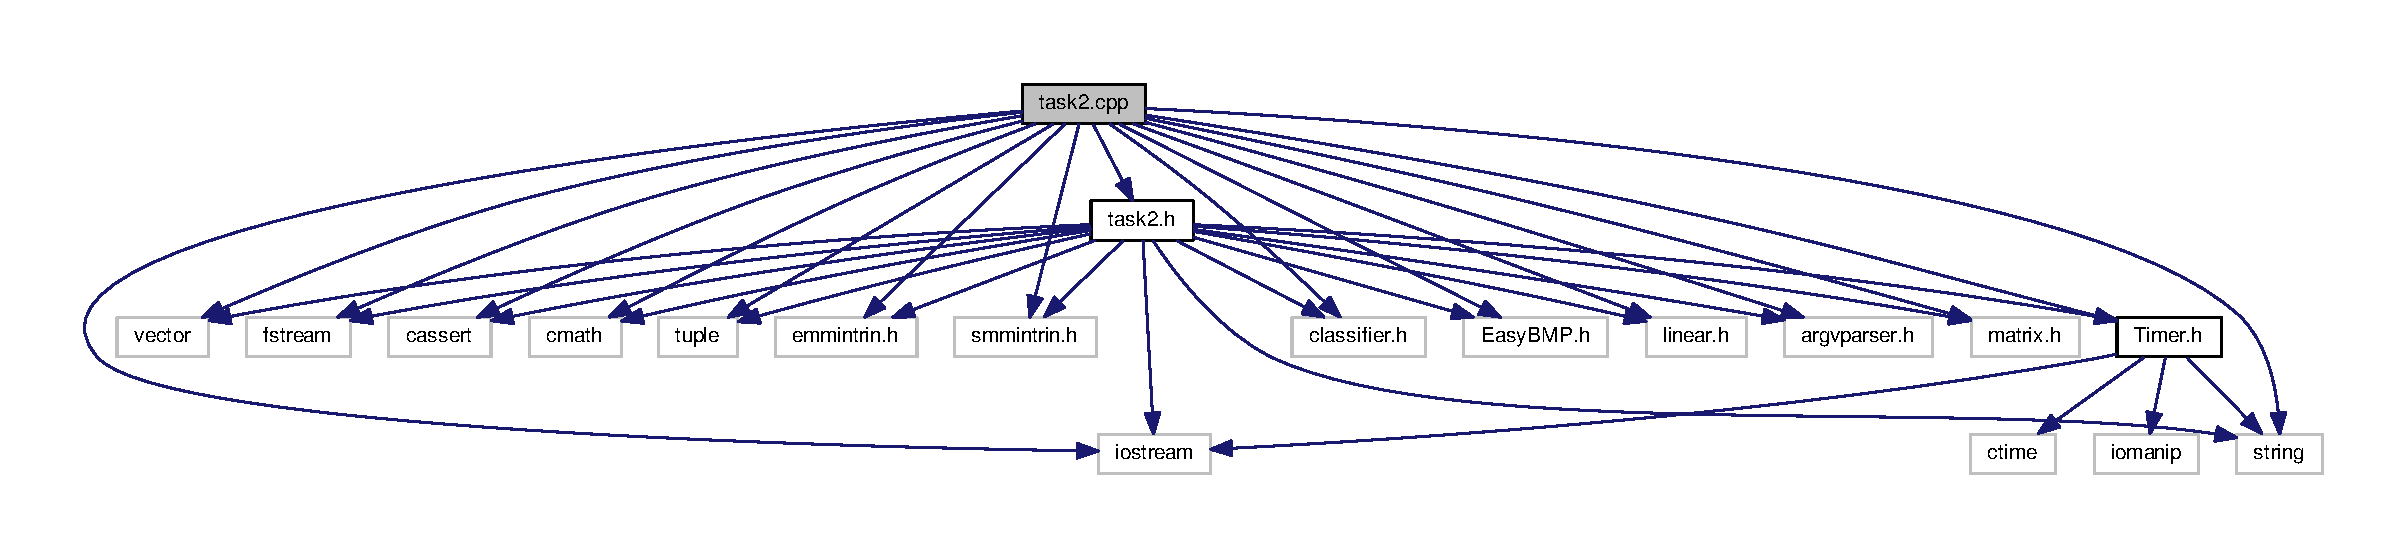
\includegraphics[width=350pt]{task2_8cpp__incl}
\end{center}
\end{figure}
\subsection*{Functions}
\begin{DoxyCompactItemize}
\item 
void \hyperlink{task2_8cpp_accaaf77285293d5ffd98febf82ca27ed}{Get4\+Pixels16\+Bit} (B\+M\+P \&in\+\_\+img, int in\+\_\+row\+\_\+idx, int in\+\_\+col\+\_\+idx, \+\_\+\+\_\+m128i $\ast$out\+\_\+\+B\+G, \+\_\+\+\_\+m128i $\ast$out\+\_\+\+R\+A)
\item 
void \hyperlink{task2_8cpp_aa1e7b0df87585a91663a6833f2c2acfe}{to\+Gray\+Scale\+S\+S\+E\+\_\+16\+B\+I\+T} (B\+M\+P \&in\+\_\+input, \hyperlink{class_my_mat}{My\+Mat}$<$ uchar $>$ \&out\+\_\+mat)
\item 
void \hyperlink{task2_8cpp_ae3f029003ab3f6ff434de3823309bd40}{Load\+File\+List} (const string \&data\+\_\+file, T\+File\+List $\ast$file\+\_\+list)
\item 
void \hyperlink{task2_8cpp_a19b69f3831c7c37fcffd448d750fa9c2}{Load\+Images} (const T\+File\+List \&file\+\_\+list, T\+Data\+Set $\ast$data\+\_\+set)
\item 
void \hyperlink{task2_8cpp_a4160a225f3ebfb369f0eac12606f0c0f}{Save\+Predictions} (const T\+File\+List \&file\+\_\+list, const T\+Labels \&labels, const string \&prediction\+\_\+file)
\item 
void \hyperlink{task2_8cpp_a6f084648182829ead67521cb1417a654}{get\+\_\+dir\+\_\+abs} (B\+M\+P $\ast$im, Matrix$<$ float $>$ \&Direct, Matrix$<$ float $>$ \&Abs)
\item 
void \hyperlink{task2_8cpp_ac0ab1652ee8133cd8416e9a2d2aa6911}{get\+\_\+dir\+\_\+abs\+\_\+\+S\+S\+E} (B\+M\+P $\ast$im, Matrix$<$ float $>$ \&Direct, Matrix$<$ float $>$ \&Abs)
\item 
void \hyperlink{task2_8cpp_ac5924a2be5d592d134ff934b8bef048c}{to\+\_\+features} (Matrix$<$ float $>$ \&Direct, Matrix$<$ float $>$ \&Abs, vector$<$ float $>$ \&one\+\_\+image\+\_\+features)
\item 
void \hyperlink{task2_8cpp_a0c9ed8baf6bec2ee28dbaceb13314004}{Extract\+Features} (const T\+Data\+Set \&data\+\_\+set, T\+Features $\ast$features, bool sse\+\_\+on)
\item 
void \hyperlink{task2_8cpp_afbd692732afb7b87860601c3355045b5}{Clear\+Dataset} (T\+Data\+Set $\ast$data\+\_\+set)
\item 
void \hyperlink{task2_8cpp_ab84e83bc0c9e229b4e28e44eab79a093}{Train\+Classifier} (const string \&data\+\_\+file, const string \&model\+\_\+file, bool sse\+\_\+on)
\item 
void \hyperlink{task2_8cpp_ac1e0c68a110dff0362b0adc7843c20a6}{Predict\+Data} (const string \&data\+\_\+file, const string \&model\+\_\+file, const string \&prediction\+\_\+file, bool sse\+\_\+on)
\item 
int \hyperlink{task2_8cpp_a3c04138a5bfe5d72780bb7e82a18e627}{main} (int argc, char $\ast$$\ast$argv)
\end{DoxyCompactItemize}


\subsection{Function Documentation}
\hypertarget{task2_8cpp_afbd692732afb7b87860601c3355045b5}{}\index{task2.\+cpp@{task2.\+cpp}!Clear\+Dataset@{Clear\+Dataset}}
\index{Clear\+Dataset@{Clear\+Dataset}!task2.\+cpp@{task2.\+cpp}}
\subsubsection[{Clear\+Dataset}]{\setlength{\rightskip}{0pt plus 5cm}void Clear\+Dataset (
\begin{DoxyParamCaption}
\item[{T\+Data\+Set $\ast$}]{data\+\_\+set}
\end{DoxyParamCaption}
)}\label{task2_8cpp_afbd692732afb7b87860601c3355045b5}
Clear dataset structure \hypertarget{task2_8cpp_a0c9ed8baf6bec2ee28dbaceb13314004}{}\index{task2.\+cpp@{task2.\+cpp}!Extract\+Features@{Extract\+Features}}
\index{Extract\+Features@{Extract\+Features}!task2.\+cpp@{task2.\+cpp}}
\subsubsection[{Extract\+Features}]{\setlength{\rightskip}{0pt plus 5cm}void Extract\+Features (
\begin{DoxyParamCaption}
\item[{const T\+Data\+Set \&}]{data\+\_\+set, }
\item[{T\+Features $\ast$}]{features, }
\item[{bool}]{sse\+\_\+on}
\end{DoxyParamCaption}
)}\label{task2_8cpp_a0c9ed8baf6bec2ee28dbaceb13314004}
Exatract features from dataset. 
\begin{DoxyParams}[1]{Parameters}
\mbox{\tt in}  & {\em data\+\_\+set} & -\/ data set with images and their class number \\
\hline
\mbox{\tt out}  & {\em features} & -\/ vector of picture descriptor and it\textquotesingle{}s class number \\
\hline
\mbox{\tt in}  & {\em sse} & -\/ enables or disables sse usage \\
\hline
\end{DoxyParams}
\hypertarget{task2_8cpp_accaaf77285293d5ffd98febf82ca27ed}{}\index{task2.\+cpp@{task2.\+cpp}!Get4\+Pixels16\+Bit@{Get4\+Pixels16\+Bit}}
\index{Get4\+Pixels16\+Bit@{Get4\+Pixels16\+Bit}!task2.\+cpp@{task2.\+cpp}}
\subsubsection[{Get4\+Pixels16\+Bit}]{\setlength{\rightskip}{0pt plus 5cm}void Get4\+Pixels16\+Bit (
\begin{DoxyParamCaption}
\item[{B\+M\+P \&}]{in\+\_\+img, }
\item[{int}]{in\+\_\+row\+\_\+idx, }
\item[{int}]{in\+\_\+col\+\_\+idx, }
\item[{\+\_\+\+\_\+m128i $\ast$}]{out\+\_\+\+B\+G, }
\item[{\+\_\+\+\_\+m128i $\ast$}]{out\+\_\+\+R\+A}
\end{DoxyParamCaption}
)\hspace{0.3cm}{\ttfamily [inline]}}\label{task2_8cpp_accaaf77285293d5ffd98febf82ca27ed}
Get4\+Pixels16\+Bit reads four consecutive pixels of the specified row started from given column and writes they to the two registers out\+\_\+\+B\+G and out\+\_\+\+R\+A. Uses 16 bit per channel 
\begin{DoxyParams}{Parameters}
{\em in\+\_\+img} & is a input image \\
\hline
{\em in\+\_\+row\+\_\+idx} & is an index of a row to read pixels \\
\hline
{\em in\+\_\+col\+\_\+idx} & ia an index of a column with a first pixel \\
\hline
{\em out\+\_\+\+B\+G} & is a pointer to a 128bit register to store blue and green channels for the pixels four consecutive pixels in format B\+B\+B\+B G\+G\+G\+G. Order of pixels is \mbox{[}0, 1, 2, 3\mbox{]} \\
\hline
{\em out\+\_\+\+R\+A} & is a pointer to a 128bit register to store red and alpha channels for the pixels four consecutive pixels in format R\+R\+R\+R A\+A\+A\+A. Order of pixels is \mbox{[}0, 1, 2, 3\mbox{]} \\
\hline
\end{DoxyParams}
\hypertarget{task2_8cpp_a6f084648182829ead67521cb1417a654}{}\index{task2.\+cpp@{task2.\+cpp}!get\+\_\+dir\+\_\+abs@{get\+\_\+dir\+\_\+abs}}
\index{get\+\_\+dir\+\_\+abs@{get\+\_\+dir\+\_\+abs}!task2.\+cpp@{task2.\+cpp}}
\subsubsection[{get\+\_\+dir\+\_\+abs}]{\setlength{\rightskip}{0pt plus 5cm}void get\+\_\+dir\+\_\+abs (
\begin{DoxyParamCaption}
\item[{B\+M\+P $\ast$}]{im, }
\item[{Matrix$<$ float $>$ \&}]{Direct, }
\item[{Matrix$<$ float $>$ \&}]{Abs}
\end{DoxyParamCaption}
)}\label{task2_8cpp_a6f084648182829ead67521cb1417a654}
get Abs and Direct matrixes without using S\+S\+E from B\+M\+P image. 
\begin{DoxyParams}[1]{Parameters}
\mbox{\tt out}  & {\em Direct} & -\/ matrix of directions \\
\hline
\mbox{\tt out}  & {\em im} & -\/ input image \\
\hline
\mbox{\tt out}  & {\em Abs} & -\/ matrix of gradient absolut values \\
\hline
\end{DoxyParams}
\hypertarget{task2_8cpp_ac0ab1652ee8133cd8416e9a2d2aa6911}{}\index{task2.\+cpp@{task2.\+cpp}!get\+\_\+dir\+\_\+abs\+\_\+\+S\+S\+E@{get\+\_\+dir\+\_\+abs\+\_\+\+S\+S\+E}}
\index{get\+\_\+dir\+\_\+abs\+\_\+\+S\+S\+E@{get\+\_\+dir\+\_\+abs\+\_\+\+S\+S\+E}!task2.\+cpp@{task2.\+cpp}}
\subsubsection[{get\+\_\+dir\+\_\+abs\+\_\+\+S\+S\+E}]{\setlength{\rightskip}{0pt plus 5cm}void get\+\_\+dir\+\_\+abs\+\_\+\+S\+S\+E (
\begin{DoxyParamCaption}
\item[{B\+M\+P $\ast$}]{im, }
\item[{Matrix$<$ float $>$ \&}]{Direct, }
\item[{Matrix$<$ float $>$ \&}]{Abs}
\end{DoxyParamCaption}
)}\label{task2_8cpp_ac0ab1652ee8133cd8416e9a2d2aa6911}
get Abs and Direct matrixes using S\+S\+E from B\+M\+P image. 
\begin{DoxyParams}[1]{Parameters}
\mbox{\tt out}  & {\em Direct} & -\/ matrix of directions \\
\hline
\mbox{\tt out}  & {\em im} & -\/ input image \\
\hline
\mbox{\tt out}  & {\em Abs} & -\/ matrix of gradient absolut values \\
\hline
\end{DoxyParams}
\hypertarget{task2_8cpp_ae3f029003ab3f6ff434de3823309bd40}{}\index{task2.\+cpp@{task2.\+cpp}!Load\+File\+List@{Load\+File\+List}}
\index{Load\+File\+List@{Load\+File\+List}!task2.\+cpp@{task2.\+cpp}}
\subsubsection[{Load\+File\+List}]{\setlength{\rightskip}{0pt plus 5cm}void Load\+File\+List (
\begin{DoxyParamCaption}
\item[{const string \&}]{data\+\_\+file, }
\item[{T\+File\+List $\ast$}]{file\+\_\+list}
\end{DoxyParamCaption}
)}\label{task2_8cpp_ae3f029003ab3f6ff434de3823309bd40}
Load list of files and its labels from \textquotesingle{}data\+\_\+file\textquotesingle{} and stores it in \textquotesingle{}file\+\_\+list\textquotesingle{} \hypertarget{task2_8cpp_a19b69f3831c7c37fcffd448d750fa9c2}{}\index{task2.\+cpp@{task2.\+cpp}!Load\+Images@{Load\+Images}}
\index{Load\+Images@{Load\+Images}!task2.\+cpp@{task2.\+cpp}}
\subsubsection[{Load\+Images}]{\setlength{\rightskip}{0pt plus 5cm}void Load\+Images (
\begin{DoxyParamCaption}
\item[{const T\+File\+List \&}]{file\+\_\+list, }
\item[{T\+Data\+Set $\ast$}]{data\+\_\+set}
\end{DoxyParamCaption}
)}\label{task2_8cpp_a19b69f3831c7c37fcffd448d750fa9c2}
Load images by list of files \textquotesingle{}file\+\_\+list\textquotesingle{} and store them in \textquotesingle{}data\+\_\+set\textquotesingle{} \hypertarget{task2_8cpp_a3c04138a5bfe5d72780bb7e82a18e627}{}\index{task2.\+cpp@{task2.\+cpp}!main@{main}}
\index{main@{main}!task2.\+cpp@{task2.\+cpp}}
\subsubsection[{main}]{\setlength{\rightskip}{0pt plus 5cm}int main (
\begin{DoxyParamCaption}
\item[{int}]{argc, }
\item[{char $\ast$$\ast$}]{argv}
\end{DoxyParamCaption}
)}\label{task2_8cpp_a3c04138a5bfe5d72780bb7e82a18e627}
Get4\+Pixels16\+Bit reads four consecutive pixels of the specified row started from given column and writes they to the two registers out\+\_\+\+B\+G and out\+\_\+\+R\+A. Uses 16 bit per channel 
\begin{DoxyParams}{Parameters}
{\em in\+\_\+img} & is a input image \\
\hline
{\em in\+\_\+row\+\_\+idx} & is an index of a row to read pixels \\
\hline
{\em in\+\_\+col\+\_\+idx} & ia an index of a column with a first pixel \\
\hline
{\em out\+\_\+\+B\+G} & is a pointer to a 128bit register to store blue and green channels for the pixels four consecutive pixels in format B\+B\+B\+B G\+G\+G\+G. Order of pixels is \mbox{[}0, 1, 2, 3\mbox{]} \\
\hline
{\em out\+\_\+\+R\+A} & is a pointer to a 128bit register to store red and alpha channels for the pixels four consecutive pixels in format R\+R\+R\+R A\+A\+A\+A. Order of pixels is \mbox{[}0, 1, 2, 3\mbox{]} \\
\hline
\end{DoxyParams}
\hypertarget{task2_8cpp_ac1e0c68a110dff0362b0adc7843c20a6}{}\index{task2.\+cpp@{task2.\+cpp}!Predict\+Data@{Predict\+Data}}
\index{Predict\+Data@{Predict\+Data}!task2.\+cpp@{task2.\+cpp}}
\subsubsection[{Predict\+Data}]{\setlength{\rightskip}{0pt plus 5cm}void Predict\+Data (
\begin{DoxyParamCaption}
\item[{const string \&}]{data\+\_\+file, }
\item[{const string \&}]{model\+\_\+file, }
\item[{const string \&}]{prediction\+\_\+file, }
\item[{bool}]{sse\+\_\+on}
\end{DoxyParamCaption}
)}\label{task2_8cpp_ac1e0c68a110dff0362b0adc7843c20a6}
Predict data from \textquotesingle{}data\+\_\+file\textquotesingle{} using model from \textquotesingle{}model\+\_\+file\textquotesingle{} and save predictions to \textquotesingle{}prediction\+\_\+file\textquotesingle{} \hypertarget{task2_8cpp_a4160a225f3ebfb369f0eac12606f0c0f}{}\index{task2.\+cpp@{task2.\+cpp}!Save\+Predictions@{Save\+Predictions}}
\index{Save\+Predictions@{Save\+Predictions}!task2.\+cpp@{task2.\+cpp}}
\subsubsection[{Save\+Predictions}]{\setlength{\rightskip}{0pt plus 5cm}void Save\+Predictions (
\begin{DoxyParamCaption}
\item[{const T\+File\+List \&}]{file\+\_\+list, }
\item[{const T\+Labels \&}]{labels, }
\item[{const string \&}]{prediction\+\_\+file}
\end{DoxyParamCaption}
)}\label{task2_8cpp_a4160a225f3ebfb369f0eac12606f0c0f}
Save result of prediction to file \hypertarget{task2_8cpp_ac5924a2be5d592d134ff934b8bef048c}{}\index{task2.\+cpp@{task2.\+cpp}!to\+\_\+features@{to\+\_\+features}}
\index{to\+\_\+features@{to\+\_\+features}!task2.\+cpp@{task2.\+cpp}}
\subsubsection[{to\+\_\+features}]{\setlength{\rightskip}{0pt plus 5cm}void to\+\_\+features (
\begin{DoxyParamCaption}
\item[{Matrix$<$ float $>$ \&}]{Direct, }
\item[{Matrix$<$ float $>$ \&}]{Abs, }
\item[{vector$<$ float $>$ \&}]{one\+\_\+image\+\_\+features}
\end{DoxyParamCaption}
)}\label{task2_8cpp_ac5924a2be5d592d134ff934b8bef048c}
get features from matrixes Abs and Direct. 
\begin{DoxyParams}[1]{Parameters}
\mbox{\tt in}  & {\em Direct} & -\/ matrix of directions \\
\hline
\mbox{\tt out}  & {\em one\+\_\+image\+\_\+features} & -\/ vector of picture descriptor and it\textquotesingle{}s class number \\
\hline
\mbox{\tt in}  & {\em Abs} & -\/ matrix of gradient absolut values \\
\hline
\end{DoxyParams}
\hypertarget{task2_8cpp_aa1e7b0df87585a91663a6833f2c2acfe}{}\index{task2.\+cpp@{task2.\+cpp}!to\+Gray\+Scale\+S\+S\+E\+\_\+16\+B\+I\+T@{to\+Gray\+Scale\+S\+S\+E\+\_\+16\+B\+I\+T}}
\index{to\+Gray\+Scale\+S\+S\+E\+\_\+16\+B\+I\+T@{to\+Gray\+Scale\+S\+S\+E\+\_\+16\+B\+I\+T}!task2.\+cpp@{task2.\+cpp}}
\subsubsection[{to\+Gray\+Scale\+S\+S\+E\+\_\+16\+B\+I\+T}]{\setlength{\rightskip}{0pt plus 5cm}void to\+Gray\+Scale\+S\+S\+E\+\_\+16\+B\+I\+T (
\begin{DoxyParamCaption}
\item[{B\+M\+P \&}]{in\+\_\+input, }
\item[{{\bf My\+Mat}$<$ uchar $>$ \&}]{out\+\_\+mat}
\end{DoxyParamCaption}
)}\label{task2_8cpp_aa1e7b0df87585a91663a6833f2c2acfe}
to\+Gray\+Scale utilizes S\+S\+E to realize fast approach to convert R\+G\+B\+A image to grayscale. It is faster than to\+Gray\+Scale\+S\+S\+E, but not so precise 
\begin{DoxyParams}[1]{Parameters}
\mbox{\tt in}  & {\em in\+\_\+input} & is an input image. \\
\hline
\mbox{\tt out}  & {\em out\+\_\+mat} & is an output image. Each pixel is represented by a single unsigned char value. \\
\hline
\end{DoxyParams}
\hypertarget{task2_8cpp_ab84e83bc0c9e229b4e28e44eab79a093}{}\index{task2.\+cpp@{task2.\+cpp}!Train\+Classifier@{Train\+Classifier}}
\index{Train\+Classifier@{Train\+Classifier}!task2.\+cpp@{task2.\+cpp}}
\subsubsection[{Train\+Classifier}]{\setlength{\rightskip}{0pt plus 5cm}void Train\+Classifier (
\begin{DoxyParamCaption}
\item[{const string \&}]{data\+\_\+file, }
\item[{const string \&}]{model\+\_\+file, }
\item[{bool}]{sse\+\_\+on}
\end{DoxyParamCaption}
)}\label{task2_8cpp_ab84e83bc0c9e229b4e28e44eab79a093}
Train S\+V\+M classifier using data from \textquotesingle{}data\+\_\+file\textquotesingle{} and save trained model to \textquotesingle{}model\+\_\+file\textquotesingle{} 
%--- End generated contents ---

% Index
\backmatter
\newpage
\phantomsection
\clearemptydoublepage
\addcontentsline{toc}{chapter}{Index}
\printindex

\end{document}
